\section{Theory} \label{sec:theory}


\subsection{Single-layer perceptron model}
The principle behind single-layer perceptrons, which is the simplest neural networks, is quite easy to understand. A set of inputs are sent into the network, and a set of outputs is returned. The inputs are multiplied by several weights, and by adjusting those weights a single perceptron can solve every \textit{linear problem} (I come back to this later). A drawing of the single-layer perceptron is found in figure (\ref{fig:single_perceptron}).

\begin{figure} [H]
	\centering
	\label{fig:single_perceptron}
	\begin{tikzpicture}
	\node[functions] (center) {};
	\node[below of=center,font=\scriptsize,text width=4em] {Activation function};
	\draw[thick] (0.5em,0.5em) -- (0,0.5em) -- (0,-0.5em) -- (-0.5em,-0.5em);
	\draw (0em,0.75em) -- (0em,-0.75em);
	\draw (0.75em,0em) -- (-0.75em,0em);
	\node[right of=center] (right) {};
	\path[draw,->] (center) -- (right);
	\node[functions,left=3em of center] (left) {$\sum$};
	\path[draw,->] (left) -- (center);
	\node[weights,left=3em of left] (2) {$o_2$} -- (2) node[input,left of=2] (l2) {$x_2$};
	\path[draw,->] (l2) -- (2);
	\path[draw,->] (2) -- (left);
	\node[below of=2] (dots) {$\vdots$} -- (dots) node[left of=dots] (ldots) {$\vdots$};
	\node[weights,below of=dots] (n) {$o_n$} -- (n) node[input,left of=n] (ln) {$x_n$};
	\path[draw,->] (ln) -- (n);
	\path[draw,->] (n) -- (left);
	\node[weights,above of=2] (1) {$o_1$} -- (1) node[input,left of=1] (l1) {$x_1$};
	\path[draw,->] (l1) -- (1);
	\path[draw,->] (1) -- (left);
	\node[weights,above of=1] (0) {$o_0$} -- (0) node[input,left of=0] (l0) {$1$};
	\path[draw,->] (l0) -- (0);
	\path[draw,->] (0) -- (left);
	\node[below of=ln,font=\scriptsize] {inputs};
	\node[below of=n,font=\scriptsize] {weights};
	\end{tikzpicture}
	\caption{Single perceptron}
	\label{fig:single_perceptron}
\end{figure}
Initially, one needs to train the network such that it knows which outputs are correct, and for that one needs to know the outputs that correspond to the inputs. Every time the network is trained, the weights are adjusted such that the error is minimized.

The very first step is to calculate the initial outputs, where the weights usually are set to small random numbers. Then the error is calculated, and the weights are updated to minimize the error. So far so good.

\subsubsection{Forward phase}\label{sec:ashortwalkthrough}
Let us look at it from a mathematical perspective, and calculate the netto output. The netto output seen from an output node is simply the sum of all the "arrows" that go to the node, see figure (\ref{fig:single_perceptron}), where each "arrow" is given by the left-hand node multiplied with its respective weight. For example the contribution from input node 2 to output node 1 follows from $X_2\cdot w_{21}$, and the total netto output to $O_1$ is therefore
\begin{equation}
net_1 = \sum_{i=1}^{I} X_i\cdot w_{i1} + b_1\cdot 1.
\end{equation}
Just some notation remarks: $X_i$ is the value of input node $i$ and $w_{ij}$ is the weight which connects input $i$ to output $j$. The vector $\vec{b}$ are the bias weights, which we will discuss later. The netto output to a node $j$ is therefore 
\begin{empheq}[box={\mybluebox[5pt]}]{equation}
net_j = \sum_{i=1}^{I} X_i\cdot w_{ij} + b_j\cdot 1.
\label{eq:forward}
\end{empheq}
You might wonder why we talk about the netto output all the time, do we have other outputs? If we look at the network mathematically, what we talk about as the netto output should be our only output. Anyway, to make the algorithm easy to implement, mapping the netto output to a final output is standard practice. You do not need to care too much about this right now, the mapping is done with an activation function and is explained further in section \ref{sec:sigmoid1}. The activation function takes in the netto output and gives the output, 
\begin{equation}
out_j = \text{sigmoid}(net_j).
\end{equation}
Now all the tools for finding the outputs are in place, and we can calculate the error. If the outputs are larger than the targets (which are the exact answers), the weights need to be reduced, and if the error is large the weights need to be adjusted a lot. The weight adjustment can be done by any minimization method, and we will look at a few gradient methods. To illustrate the point, we will stick to the \textbf{gradient descent} (GD) method in the calculations, even though other methods will be used later. The principle of GD is easy: each weight is "moved" in the direction of steepest slope,
\begin{empheq}[box={\mybluebox[5pt]}]{equation}
w_{ij}^+= w_{ij} - \eta\cdot\frac{\partial E_{TOT}}{\partial w_{ij}},
\label{eq:w_update}
\end{empheq}
where $\eta$ is what we call the learning rate. If not everything is clear right now, it is fine. We will discuss the most important concepts before we dive into the maths.

\subsubsection{BIAS}
As mentioned above, we use biases when calculating the outputs. The nodes, with value $B$, are called the bias nodes, and the weights, $b$, are called the bias weights. But why do we need those? 

Suppose we have two inputs of value zero, and one output which should not be zero (this could for instance be a NOR gate). Without the bias, we will not be able to get any other output than zero, and in fact the network would struggle to find the right weights even if the output had been zero. 

The bias value $B$ does not really matter since the network will adjust the bias weights with respect to it, and is usually set to 1 and ignored in the calculations.

\subsubsection{Learning rate}
In principle, the weights could be updated without adding any learning rate ($\eta=1$), but this can in practice be problematic. It is easy to imagine that the outputs can be fluctuating around the targets without decreasing the error, which is not ideal, and a learning rate can be added to avoid this. The downside is that with a low learning rate the network needs more training to obtain the correct results (and it takes more time), so we need to find a balance. 

\subsubsection{Cost function}\label{sec:error_function}
The cost function we will use is inspired by the error function used in \textbf{least squares methods}, and reads
\begin{empheq}[box={\mybluebox[5pt]}]{equation}
E_{TOT} = \frac{1}{2}\sum_j (y_j - t_j)^2
\label{eq:error_function}
\end{empheq}
where we sum over all the outputs. The factor $1/2$ is added just to give a clean derivative, which in fact makes all the expressions neater. It would also be possible to use other error functions, but to find specific expressions for the weight updating formulas, we better focus on the one above. 

\subsubsection{Activation function}\label{sec:sigmoid1}
Inspired by Boolian algebra, the inputs and outputs initially are set to either 0, 1, or a superposition of them. To ensure that every output is between 0 and 1, we map them all using a cost function. Perhaps the most common function to use is
\begin{empheq}[box={\mybluebox[5pt]}]{equation}
f(x)=\frac{1}{1+\exp(-x)}
\label{eq:sigmoid}
\end{empheq}
which maps between 0 and 1 as required. Another important property is that the derivative of this function has an easy form, which is important. The derivative of this function is
\begin{equation}
f'(x)=f(1-f)
\end{equation}
and the derivation of it is shown carefully in Appendix A. The function is presented in figure (\ref{fig:sigmoid1}).
\begin{figure} [H]
	\centering
	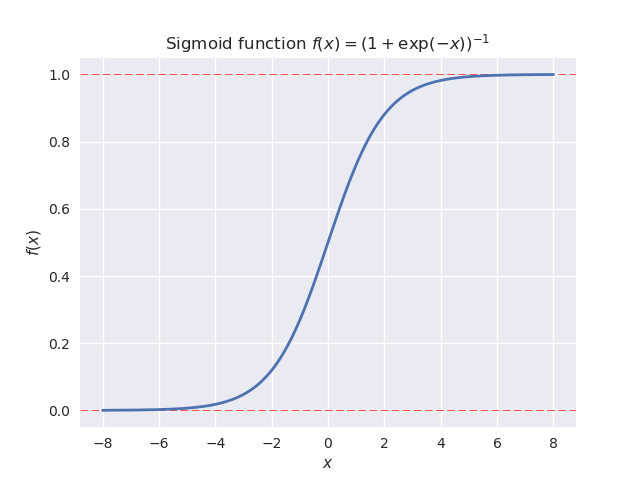
\includegraphics[scale=0.65]{images/sigmoid1.png}
	\caption{A sigmoid function plotted from -8 to 8. The asymptotes are drawn to stress that the function will approach the value 1 when $x\rightarrow \infty$ and the value 0 when $x\rightarrow -\infty$.}
	\label{fig:sigmoid1}
\end{figure} 

Examples on other activation functions are \textit{tanh, standard RELU, leaky RELU and ELU}. 

\subsubsection{Backward phase}
Now we have the fundamentals to go further with the theory expressed in section \ref{sec:ashortwalkthrough}. Actually, the only thing we are left with is finding an expression for the weight updating based on the formula from equation (\ref{eq:w_update}), where the partial derivative is what we need to find. The computations are in detail done in Appendix B, and we obtain the equations
\begin{empheq}[box={\mybluebox[5pt]}]{align}
w_{ij}^{+}&=w_{ij} + \eta\cdot(t_j-out_j)\cdot out_j(1-out_j)\cdot X_i\\
b_i^+&=b_i + \eta\cdot(t_i-out_i)\cdot out_i(1-out_i)
\end{empheq}
for updating the weights and bias weights respectively. Then and all the basics for the single perceptron are set. 

\subsubsection{Constraints}
It is naturally that such a simple algorithm has constraints, and in fact it is only able to solve so-called linear problems. The logic functions, such as OR, NOR, AND and NAND are common examples, which all can be implemented using a single perceptron. On the other hand, the single perceptron is not capable of recognize non-linear functions, such as the XOR-gate.



\subsection{Multilayer perceptron model}
If you have understood the single perceptron, 
In fact, every problem can be solved by a two-layer perceptron, according to \textbf{the universal approximation theorem}. However, in many cases we do not know how many nodes that are sufficient, and it might be just as smart to add another layer to ensure that you have enough weights. 

Start with 2-layer neural network\\
\begin{figure}[H]
	\centering
	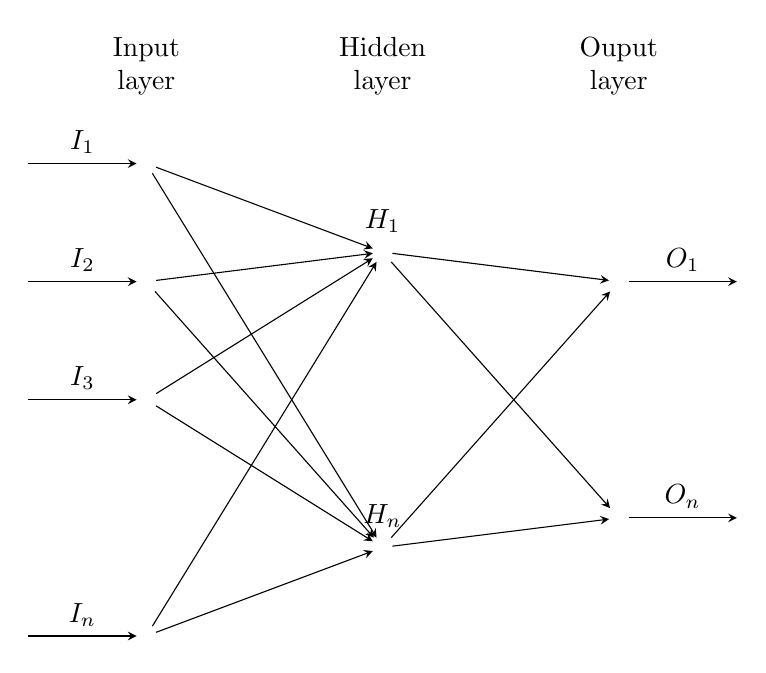
\begin{tikzpicture}[x=1.5cm, y=1.5cm, >=stealth]
	
	\foreach \m/\l [count=\y] in {1,2,3,missing,4}
	\node [every neuron/.try, neuron \m/.try] (input-\m) at (0,2.5-\y) {};
	
	\foreach \m [count=\y] in {1,missing,2}
	\node [every neuron/.try, neuron \m/.try ] (hidden-\m) at (2,2-\y*1.25) {};
	
	\foreach \m [count=\y] in {1,missing,2}
	\node [every neuron/.try, neuron \m/.try ] (output-\m) at (4,1.5-\y) {};
	
	\foreach \l [count=\i] in {1,2,3,n}
	\draw [<-] (input-\i) -- ++(-1,0)
	node [above, midway] {$I_\l$};
	
	\foreach \l [count=\i] in {1,n}
	\node [above] at (hidden-\i.north) {$H_\l$};
	
	\foreach \l [count=\i] in {1,n}
	\draw [->] (output-\i) -- ++(1,0)
	node [above, midway] {$O_\l$};
	
	\foreach \i in {1,...,4}
	\foreach \j in {1,...,2}
	\draw [->] (input-\i) -- (hidden-\j);
	
	\foreach \i in {1,...,2}
	\foreach \j in {1,...,2}
	\draw [->] (hidden-\i) -- (output-\j);
	
	\foreach \l [count=\x from 0] in {Input, Hidden, Ouput}
	\node [align=center, above] at (\x*2,2) {\l \\ layer};
	
	\end{tikzpicture}
	\caption{...}
\end{figure}

For the single perceptron the updating of weights was quite straight forward, but for a perceptron consisting of multiple layers the question is: how do we update the weights when we do not know the value of the hidden nodes? And how do we know which layer that causes the error? This will be explained in the next subsection, where one of the most popular techniques for this is taken into account.

\subsubsection{Backward Propagation}
Backward propagation is probably the most used technique to update the weights, and is actually again based on equation (\ref{eq:w_update}). What differs the 

We recognize the first part as $\delta_{ok}$, such that
\begin{empheq}[box={\mybluebox[5pt]}]{equation}
w_{ij}^{(1)}\rightarrow w_{ij}^{(1)} - \eta\cdot\sum_{k=1}^{O}\delta_{ok}\cdot w_{jk}^{(2)}\cdot out_{hj}(1-out_{hj})\cdot x_i
\end{empheq}
where we recall $\delta_{ok}$ as
\begin{equation*}
\delta_{ok}=-(t_{ok}-out_{ok})\cdot out_{ok}(1-out_{ok}).
\end{equation*}

\subsubsection{Manymany layers}
Since it will be quite a lot calculations, I will just express the results here, and move the calculations to Appendix C. Let us start with the forward propagation:
\begin{empheq}[box={\mybluebox[5pt]}]{align}
net_{hi}&=\sum_jw_{ji}^{(1)}\cdot i_j + b_{1i}\cdot 1\notag\\
out_{hi}&=\text{sig}(net_{hi})\notag\\
\notag\\
net_{ki}&=\sum_jw_{ji}^{(2)}\cdot out_{hj} + b_{2i}\cdot 1\\
out_{ki}&=\text{sig}(net_{ki})\notag\\
\notag\\
net_{oi}&=\sum_jw_{ji}^{(3)}\cdot out_{kj} + b_{3i}\cdot 1\notag\\
out_{oi}&=\text{sig}(net_{oi})\notag
\end{empheq}
which can easily be turned into vector form. The backward propagation follows from the two-layer example, and we get
\begin{empheq}[box={\mybluebox[5pt]}]{align}
w_{ij}^{(3)}&=w_{ij}^{(3)}-\eta\cdot\delta_{oj}\cdot out_{ki}\notag\\
\notag\\
w_{ij}^{(2)}&=w_{ij}^{(2)}-\eta\sum_{k=1}^O\delta_{ok}\cdot w_{jk}^{(3)}\cdot out_{kj}(1-out_{kj})\cdot out_{hi}\notag\\
\notag\\
w_{ij}^{(1)}&=w_{ij}^{(1)}-\eta\sum_{k=1}^O\sum_{l=1}^K\delta_{ok}\cdot w_{lk}^{(3)}\cdot out_{kl}(1-out_{kl})\cdot w_{jl}^{(2)}out_{hj}(1-out_{hj})\cdot x_i\notag
\end{empheq}
where we again use the short hand 
\begin{equation*}
\delta_{oj}=(t_j-out_{oj})\cdot out_{oj}(1-out_{oj}).
\end{equation*}
If we compare with the weight update formulas for the two-layer case, we recognize some obvious connections, and it is easy to imagine how we can construct a general weight update algorithm, no matter how many layers we have. 